\chapter{Genetic Algorithms}

The previous three chapters showed you how to write Unicon programs with
many kinds of Internet and system capabilities that are expected of
most modern applications. Unicon is great for generic computing tasks,
but it really excels when its advanced features are applied in
application areas where the development of the algorithms is complex.
This chapter describes how to use Unicon to build an entire, somewhat
complex application with reusable parts. The field of \index{genetic
algorithms}\textit{genetic algorithms} (GAs) is an exciting application
domain with lots of opportunities for exploratory programming. When
you're finished with this chapter, you will 
\begin{itemize}
\item Understand the basics of genetic algorithms.
\item See how to build genetic algorithm engine in Unicon.
\item Use that GA engine to build programs for your own projects.
\end{itemize}

\section{What are Genetic Algorithms?}

The broad field of evolutionary computation has been an area of active
research since the 1950s. Initially, it was led by computer scientists
that believed evolution could be used as an optimization tool for
engineering problems. Genetic Programming (GP) focuses on evolving
computer programs to perform various tasks. On the other hand, GAs
focus on the simpler task of evolving data that is used to solve a
problem. The GAs that we'll study have a binary
representation. Increasingly there has been a shift towards non-binary
representations such as floating-point numbers in GA-related projects.
That field has typically been given the more general name of
evolutionary algorithms. GAs have one of the most well-defined
mathematical foundations in all of evolutionary computation, and are a
good place to start exploring. 

John Holland invented the first GAs in the 1960s. His goal was to study
adaptation as it occurs in nature and then to create computer systems
to model the adaptive process. Holland combined four elements that are
common to all GAs:

\begin{itemize}
\item A population of individuals
\item Selection based on fitness
\item Mating of individuals
\item Random mutation
\end{itemize}
Consider the very simple problem of finding the largest number encoding
in binary with six digits. Assume the GA knows nothing about binary
encoding.

While making use of a population might seem to be a necessary element
for any evolutionary computation, it is not. Instead, you could focus
all your efforts on improving one individual. In this case, fitness is
exactly the numerical value of an individual. For example, you could
examine the fitness of this one individual with an exhaustive search:

\iconcode{
\>   best := 0 \\
\>   every i := 0 to 2\^{}6 do \\
\>   \ \ \ best {\textless}:= i
}

Suppose you only make use of the elements of a population and selection
based on fitness. You could have a population of six individuals,
randomly initialized, and you could attempt to improve the overall
fitness of the six by replacing the lowest fitness individual with a
random one. The code below shows how to implement this idea:

\iconcode{
\>   maxi := 2\^{}6 \\
\>   population := [?maxi, ?maxi, ?maxi, ?maxi, ?maxi, ?maxi] \\
\>   every i := 1 to 100 do \{ \\
\>   \ \ \ worst := 1 \\
\>   \ \ \ every i := 1 to 5 do \\
\>   \ \ \ \ \ \ if population[worst] {\textless}= population[i] then \\
\>   \ \ \ \ \ \ \ \ \ worst := i \\
\>   \ \ \ population[i] := ?maxi \\
\>   \ \ \ \}
}

Before modeling mating and mutation, you'll have to
create a more detailed representation of the internals of an
individual.

\section{Operations: Fitness, Crossover, and Mutation}

An individual is represented by a string from a binary alphabet.
Incidentally, natural evolution of DNA is based on a quaternary
alphabet, but the size of the alphabet is unimportant for a computer
model. In Unicon, you could represent these individuals with lists of
integers. However, strings of \texttt{"1"}
and \texttt{"0"} characters provide a
representation that is easier to use. So, here is a more explicit
representation of a population:

\iconcode{
\>   population := ["010111", "000101", "111101", "111011", "111110", "010110"]
}

\subsection*{Fitness}

The fitness can be computed by converting the string representation into
an integer as follows: \texttt{integer("2r"
{\textbar}{\textbar} population[1])}. The \texttt{2r} means that this
is a literal representation of an integer in base two form. There are
many different possible selection schemes used in GAs. This chapter
uses one that has proven to be very robust in a large number of
different GA applications, called \textit{tournament selection}. The
general idea is to group the individuals and have them compete
head-to-head. The winners of the tournaments are selected to live in
the next generation; their bits are copied into an element in the new
population. Tournaments of size two work well. All you must do is
randomly pair up the individuals, and move the one with the higher
fitness to the next generation. Because you generally will want the
population size to remain constant, you'll have to do
this pairing twice. Here is a tournament selection on the above
population:

\iconcode{
\>   population[1] := "010111"
\# 23 winner \\
\>   population[6] := "010110"
\# 22 \\
\>   population[3] := "111101"
\# 61 winner \\
\>   population[4] := "111011"
\# 59 \\
\>   population[5] := "111110"
\# 62 winner \\
\>   population[2] := "000101"
\# 5
}

The second round of selections is listed here:

\iconcode{
\>   population[5] := "111110"
\# 62 winner \\
\>   population[6] := "010110"
\# 22 \\
\>   population[2] := "000101"
\# 5 \\
\>   population[3] := "111101"
\# 61 winner \\
\>   population[4] := "111011"
\# 59 winner \\
\>   population[1] := "010111"
\# 23
}

The end result of tournament selection is listed here:

\iconcode{
\>   next\_gen[1] := population[1] :=
"010111" \# 23 \\
\>   next\_gen[2] := population[3] :=
"111101" \# 61 \\
\>   next\_gen[3] := population[5] :=
"111110" \# 62 \\
\>   next\_gen[4] := population[5] :=
"111110" \# 62 \\
\>   next\_gen[5] := population[3] :=
"111101" \# 61 \\
\>   next\_gen[6] := population[4] :=
"111011" \# 59
}

Notice how there are two copies of \texttt{population[3]} and
\texttt{population[5]} in \texttt{next\_gen}. On the other hand, there
are no copies of \texttt{population[2]}.

\subsection*{Crossover}

Mating, more technically known as crossover, involves the sharing of
information between members of the population. Again there are many
different types of mating schemes, but this chapter describes one
called two-point crossover (Figure 17-1) that has proven to be very
robust for a wide range of GA applications. Once again, randomly pair
up the individuals, but this time instead of competing, individuals
will mate. First you must transform the linear strings into circular
rings. For each pair, randomly select two points in the ring and cut
the rings at the two selected points. Then swap the ring segments to
form two new rings.\\


\begin{center}
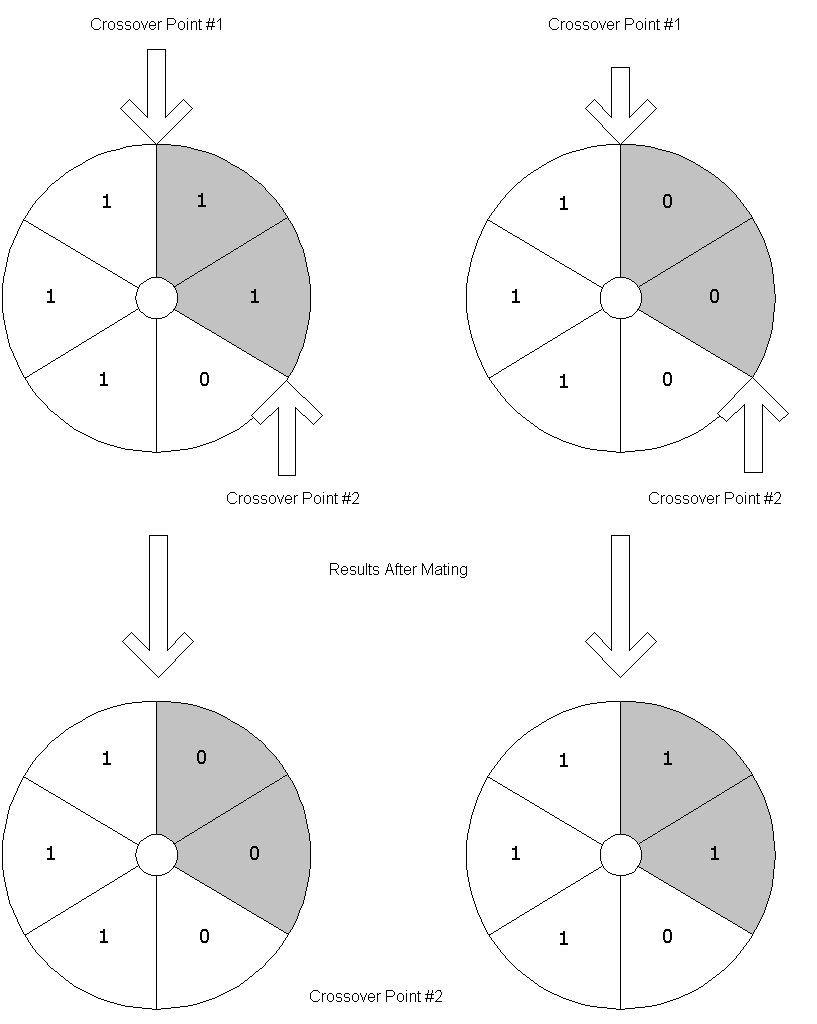
\includegraphics[width=3.322in,height=3.9453in]{ub-img/ub-img45.png}
\end{center}

{\sffamily\bfseries Figure 17-1:}
{\sffamily Two-point crossover.}

The code for two-point crossover is presented below. The
\texttt{?(lchrom+1)} expression picks a random number between one and
the length of the chromosome. Variables \texttt{a} and \texttt{b} are
initialized to two different values in this range; \texttt{a} is made
the smaller of the two indices. Two children in the new generation are
formed by splicing portions of \texttt{parent1} and \texttt{parent2}
within the range from \texttt{a} to \texttt{b}.

\iconcode{
\>   \ \ \ a := ?(lchrom+1) \\
\>   \ \ \ while ((b := ?(lchrom+1)) = a) \\
\>   \ \ \ if a {\textgreater} b then a :=: b \\
\>   \ \ \ ncross +:= 1 \\
\>   \ \ \ child1 := parent1[1:a] {\textbar}{\textbar} parent2[a:b]
{\textbar}{\textbar} parent1[b:0] \\
\>   \ \ \ child2 := parent2[1:a] {\textbar}{\textbar} parent1[a:b]
{\textbar}{\textbar} parent2[b:0]
}

\subsection*{Mutation}

The last GA operation is mutation. Mutation works at the independent
level of single binary digits. To implement mutation, take a look at
each bit of each individual of the population. With a fixed
probability, flip the value of the bit. This is the basic mechanism for
injecting completely new information into the population. Almost all of
that information will be useless, but as the GA evolves it will weed
out the useless information and keep the useful information. 

\section{The GA Process}

Now that you have a handle on the basic operations, it is time to
describe the basic GA algorithm for applying these operations. 

\ \ 1.\ \ Generate a random population of n individuals each with
\textit{l}{}-bits.

\ \ 2.\ \ Calculate the fitness of each individual.

\ \ 3.\ \ Perform tournament selection on the population to produce a
new generation.

\ \ 4.\ \ With probability p\textsubscript{c}, mate pairs of individuals
using two-point crossover.

\ \ 5.\ \ With probability p\textsubscript{m}, mutate the bits in the
population.

\ \ 6.\ \ Replace the old population with the new generation.

\ \ 7.\ \ Go to step 2, until the population meets some desired
condition.

Even with this mechanical algorithm, applying a GA to any specific
problem remains an art. For example, step 7 leaves the desired
stopping condition up to the implementer. Typically the stopping
condition might be something like: until the average fitness has not
risen significantly in the last five generations. This is one of
many implementation choices you have to make,
from variations on crossover to adjusting the
mutation and mating rates. Here are some time-tested rules of thumb:

\ \ 1.\ \ Encode the solutions to a problem with as few bits as possible
but not at the expense of making the encoding very complex. 

\ \ 2.\ \ Let the size of the population be at least twenty but not so
large that your computer program is intolerably slow. 

\ \ 3.\ \ Mating rates between 30 percent and 90 percent work for a
large range of problems.

\ \ 4.\ \ Mutation rates should be near 1/\textit{(the number of bits)},
so that each
individual undergoes about one mutation on average per generation.

\ \ 5.\ \ Once the average fitness of the population does not change
significantly after ten generations, the population has converged on
the solution. At this point, stop the GA and study the population of
solutions.


\section{\texttt{ga\_eng}: a Genetic Algorithm Engine}

The \texttt{ga\_eng} engine is a general purpose reusable GA engine that
can quickly and easily be adapted to solve a variety of problems. This
section presents its key elements. The full \index{source code}source
code for \texttt{ga\_eng} is on the book's web site.

From the preceding sections, you can tell that a GA maintains a large
amount of information as it transitions from one generation to the
next. What is the state information that the engine needs to track?
\ Below is a list of the most obvious things to record:

\begin{itemize}
\item n $-$ the size of the population
\item \textit{l} $-$ the length of the individual's bit
representation
\item p\textsubscript{c} $-$ the probability of crossover mating
\item p\textsubscript{m} $-$ the probability of mutation
\item population $-$ a list of a current population's
individuals
\end{itemize}
Given the above state information, what can a GA engine do?

\begin{itemize}
\item \texttt{init()} $-$ initialize the state information and
population
\item \texttt{evolve()} $-$ move a population from one generation to the
next
\item \texttt{tselect()} $-$ perform tournament of selection on the
population
\item \texttt{stats()} $-$ collect statistics about the current
population to monitor progress
\end{itemize}

\subsection*{The fitness function}

A key application-specific interface issue is the fitness function. The
user of the GA engine sets the fitness values of each member of the
population. If that value is not set, the default value will be the
average of the fitness of each of the parents. Each
parent's contribution to the fitness is weighted by
how many bits it contributed to the offspring. This has the nice
property of not requiring that each individual's
fitness be computed at every generation.

To use the GA engine, the programmer supplies an application-specific
fitness function \texttt{f(x)} that is applied to each individual of
the population every generation. Given a binary string \texttt{s},
\texttt{f(s)} would return a numeric fitness value.

\subsection*{Methods and attributes of class \texttt{ga\_eng}}

Class \texttt{ga\_eng} implements the engine. It provides
two public methods, \texttt{evolve()} and \texttt{set\_params()}, as
well as eight private methods: 

\iconcode{
method evolve() \\
method set\_params(fitness\_func, popsize, lchrom, pcross, pmutation, log\_file) \\
method tselect() \\
method crossover2(parent1, parent2) \\
method generation() \\
method stats(Pop) \\
method report(Pop) \\
method random\_chrom() \\
method initpop() \\
method init()
}

The \texttt{set\_params()} method sets the fitness function, the
population size, the length of the chromosomes, the probability of
crossover, the probability of mutation, and the log file for generating
a trace of \ a run. The \index{constructor}constructor
\texttt{ga\_eng()} takes the same input parameters as
\texttt{set\_params()} but it also re-initializes the engine by
creating a new population from scratch. The \texttt{evolve()} method
moves the population from one generation to the next.

The \texttt{tselect()} method operates on the whole population by
performing tournament selection. The \texttt{crossover2()} method takes
two individuals and returns two new individuals in a list after doing
two-point crossover. The \texttt{stats()} method collects statistics on
the given population, and \texttt{report()} writes the results out to
the log file if it is not set to \texttt{\&null}. The \texttt{init()}
and \texttt{initpop()} methods initialize the GA.

You might be asking what is a population of \textit{individuals}? \ The
key pieces of information about an individual are its chromosomes,
which are represented as a string of zeros and ones. For implementation
reasons, we bundle the following information for each individual using
the following Unicon record: 

\iconcode{
record individual(chrom, fitness, parent1, parent2, xsite)}

This stores the fitness values, the index of two parents, and the
crossover sites from when the parents were mated.

The class \texttt{ga\_eng} makes use of the following
\index{instance}instance variables: 

\begin{itemize}
\item \texttt{oldpop}, \texttt{newpop} $-$ two populations; selection
goes from \texttt{oldpop} into \texttt{newpop}
\item \texttt{popsize}, \texttt{lchrom} $-$ the population size and the
length of the chromosomes
\item \texttt{gen}, \texttt{maxgen} $-$ current and max generation
number
\item \texttt{pcross}, \texttt{pmutation} $-$ the probability of
crossover and mutation
\item \texttt{sumfitness} $-$ the sum of the fitness of the entire
population
\item \texttt{nmutation} $-$ number of mutation in the current
generation
\item \texttt{ncross} $-$ number of crossovers (or matings) in the
current generation
\item \texttt{avg}, \texttt{max}, \texttt{min} $-$ average, maximum, and
minimum fitness in the population
\item \texttt{best} $-$ the location of the individual with the highest
fitness
\item \texttt{log\_file} $-$ a text file where statistics are written
during a GA run
\item \texttt{fitness\_func} $-$ the user-supplied fitness function. It
reads a string of zeros and ones and returns a number representing the
fitness.
\end{itemize}


\subsection*{A Closer Look at the \texttt{evolve()} method}

Space limitations preclude discussing every method of
\texttt{ga\_eng}, but \texttt{evolve()} is a method that is called
by user code, and defines the basic architecture of the
engine. The \texttt{evolve()} method initializes the population the
first time the method is invoked by each instance of \texttt{ga\_eng}.
After initialization and in subsequent calls, \texttt{evolve()}
does three things: it collects statistics, writes the results to a log
file, and then evolves the population for one generation. The method
\texttt{generation()} then becomes the focus of activity. The code for
\texttt{evolve()} is:

\iconcode{
method evolve() \\
\>   if /initialized := 1 then \{ \\
\>\>    gen := 0 \\
\>\>    init() \\
\>\>    statistics(oldpop) \\
\>\>    if {\textbackslash}log\_file then report(oldpop) \\
\>\>    \} \\
\>   gen +:= 1 \\
\>   generation() \\
\>   statistics(newpop) \\
\>   if {\textbackslash}log\_file then report(newpop) \\
\>   oldpop := newpop \\
end
}

Generation consists of three high-level operations. Tournament
selection is performed via a call to \texttt{tselect()}, which makes
copies of selected individuals from \texttt{oldpop} to
\texttt{newpop}.
After this, all operations take place on individuals in
\texttt{newpop}. The next two operations are performed in a
loop, on pairs of individuals. The \texttt{crossover2()} method does
the mating; it encapsulates the relatively low-level operation of
mutation. The last high-level operation that a GA does is call the user
supplied \texttt{fitness\_func} to assign a fitness value to each
individual in the new population. The GA keeps track of only two
generations for the \texttt{evolve()} method to continue as long as
needed. Once each individual has been evaluated, that generation is
complete. The \texttt{oldpop} variable is assigned the value of the
\texttt{newpop}, and the process is ready to start again. Listing 17-1
shows the code for the method \texttt{generation()}:

\bigskip

{\sffamily\bfseries Listing 17-1}

{\sffamily\bfseries A method for producing a new generation.}

\iconcode{
method generation() \\
\>   local j := 1, mate1, mate2, jcross, kids, x, fitness1, fitness2, selected
\\
\>   newpop \ \ \ := list(popsize) \\
\>   nmutation := ncross := 0 \\
\>   selected \ \ := tselect() \\
\>   repeat \ \{ \\
\>   \ \ \ mate1 := selected[j] \\
\>   \ \ \ mate2 := selected[j+1] \\
\>   \ \ \ kids := crossover2(oldpop[mate1].chrom, oldpop[mate2].chrom ) \\
\>   \ \ \ fitness1 := fitness\_func(oldpop[mate1].chrom) \\
\>   \ \ \ fitness2 := fitness\_func(oldpop[mate2].chrom) \\
\>   \ \ \ newpop[j]:= individual(kids[1], fitness1, mate1, mate2, kids[3]) \\
\>   \ \ \ newpop[j+1] := individual(kids[2], fitness2, mate1, mate2, kids[3])
\\
\>   \ \ \ if j {\textgreater} popsize then break \\
\>   \ \ \ j +:= 2 \\
\>   \ \ \ \} \\
end
}

\subsection*{Using \texttt{ga\_eng}}

GAs are extremely robust. It is easy to create a buggy GA that
works so well that the bugs go undetected. Masking of
bugs by robust algorithms is not unique to GA; it occurs in many
numerical algorithms. To prevent this, the following code tests
the GA on a simple problem where having one bit increases the fitness
values by one. This is a ready to compile and run GA application,
albeit a very simple one. As you can see, \texttt{ga\_eng()} and
\texttt{evolve()} are all the interface methods you need to build a
complete genetic algorithm. Listing 17-2 shows all the code needed
to use the GA engine for a simple test problem.

\bigskip

{\sffamily\bfseries Listing 17-2}

{\sffamily\bfseries Using \texttt{ga\_eng()} for a simple test problem}

\iconcode{
procedure decode(chrom) \\
\>   local i := 0 \\
\>   every !chrom == "1" do i +:= 1 \\
\>   return i \\
end \\
\ \\
\# a simple test of the engine, fitness is based on number of 1 bits in chrom \\
procedure main() \\
\>   log\_file \ := open("test\_ga.log",
"w") {\textbar} stop("cannot open log\_file.log") \\
\>   ga := ga\_eng(decode, 100, 20, 0.99, 1.0/real(20), log\_file) \\
\>   every 1 to 100 do ga.evolve() \\
\>   write(log\_file, "best location ={\textgreater} ", ga.best) \\
\>   write(log\_file, "best fitness \ ={\textgreater} ",
           ga.newpop[ga.best].fitness) \\
end
}

\subsection*{Log files}

The log file \texttt{test\_ga.log} contains a lot of statistics. Listing
17-3 is a fragment of the log file that is generated. The complete log
file has over twelve thousand lines.

\bigskip

{\sffamily\bfseries
Listing 17-3}

{\sffamily\bfseries
A trace of the GA for a simple test problem}


\iconcode{
Log\_File for Genetic Algorithm (GA) \\
\ \\
\ Population size \ \ \ \ \ \ \ \ \ = 100 \\
\ Chromosome length \ \ \ \ \ \ \ = 20 \\
\ Maximum \# of generations =  \\
\ Crossover probability \ \ \ = 0.99 \\
\ Mutation probability \ \ \ \ = 0.05 \\
\ \\
\ Initial population maximum fitness = \ 5.00e-1  \\
\ Initial population average fitness = \ 5.00e-1  \\
\ Initial population minimum fitness = \ 5.00e-1  \\
\ Initial population sum of \ fitness = \ 5.00e1 \  \\
{}-{}-{}-{}-{}-{}-{}-{}-{}-{}-{}-{}-{}-{}-{}-{}-{}-{}-{}-{}-{}-{}-{}-{}-{}-{}-{}-{}-{}-{}-{}-{}-{}-{}-{}-{}-{}-{}-{}-{}-{}-{}-{}-{}-{}-{}-{}-{}-{}-{}-{}-{}-{}-{}-{}-{}-{}-{}-{}-{}- \\
Population Report \\
\>   \ \ \ \ \ \ \ \ \ \ \ \ \ \ \ \ \ \ \ \ \ \ \ \ \ \ \ Generation 0 \\
\ \\
\>   \ \ \# \ \ \ parents \ \ \ \ \ \ xsite \ \ chromo
\ \ \ \ \ \ \ \ \ \ \ \ \ \ \ fitness \\
{}-{}-{}-{}-{}-{}-{}-{}-{}-{}-{}-{}-{}-{}-{}-{}-{}-{}-{}-{}-{}-{}-{}-{}-{}-{}-{}-{}-{}-{}-{}-{}-{}-{}-{}-{}-{}-{}-{}-{}-{}-{}-{}-{}-{}-{}-{}-{}-{}-{}-{}-{}-{}-{}-{}-{}-{}-{}-{}-{}- \\
\ \ \ \ \ \ \ 1) ( \ 0, \ \ 0) \ \ \ \ \ \ 0 \ \ \ 00010001110001000010
\ 5.00e-1  \\
\ \ \ \ \ \ \ 2) ( \ 0, \ \ 0) \ \ \ \ \ \ 0 \ \ \ 11011101011010001100
\ 5.00e-1  \\
\ \ \ \ \ \ \ 3) ( \ 0, \ \ 0) \ \ \ \ \ \ 0 \ \ \ 01101100000110100111
\ 5.00e-1  \\
..........  \\
\>   \ \ 100) ( \ 0, \ \ 0) \ \ \ \ \ \ 0 \ \ \ 11011100110011001010
\ 5.00e-1  \\
{}-{}-{}-{}-{}-{}-{}-{}-{}-{}-{}-{}-{}-{}-{}-{}-{}-{}-{}-{}-{}-{}-{}-{}-{}-{}-{}-{}-{}-{}-{}-{}-{}-{}-{}-{}-{}-{}-{}-{}-{}-{}-{}-{}-{}-{}-{}-{}-{}-{}-{}-{}-{}-{}-{}-{}-{}-{}-{}-{}- \\
Statistics:  \\
min = \ 5.00000000e-1 \ avg = \ 5.00000000e-1 \ max = \ 5.00000000e-1  \\
\ no. of mutations \ \ \ \ \ \ \ = 0 \\
\ no. of crossovers \ \ \ \ \ \ = 0 \\
\ location of best chromo = 1 \\
{}-{}-{}-{}-{}-{}-{}-{}-{}-{}-{}-{}-{}-{}-{}-{}-{}-{}-{}-{}-{}-{}-{}-{}-{}-{}-{}-{}-{}-{}-{}-{}-{}-{}-{}-{}-{}-{}-{}-{}-{}-{}-{}-{}-{}-{}-{}-{}-{}-{}-{}-{}-{}-{}-{}-{}-{}-{}-{}-{}- \\
dateline = Wednesday, January 27, 1999 \ 10:37 pm \\
................. \\
Population Report \\
\>   \ \ \ \ \ \ \ \ \ \ \ \ \ \ \ \ \ \ \ \ \ \ \ \ \ \ \ Generation
100 \\
\ \\
\>   \ \ \# \ \ \ parents \ \ \ \ \ \ xsite \ \ chromo
\ \ \ \ \ \ \ \ \ \ \ \ \ \ \ fitness  \\
{}-{}-{}-{}-{}-{}-{}-{}-{}-{}-{}-{}-{}-{}-{}-{}-{}-{}-{}-{}-{}-{}-{}-{}-{}-{}-{}-{}-{}-{}-{}-{}-{}-{}-{}-{}-{}-{}-{}-{}-{}-{}-{}-{}-{}-{}-{}-{}-{}-{}-{}-{}-{}-{}-{}-{}-{}-{}-{}-{}- \\
\ \ \ \ \ \ \ 1) ( \ 1, \ \ 2) \ \ 15:21 \ \ \ 00011011011000010100
\ 9.19e0 \  \\
\ \ \ \ \ \ \ 2) ( \ 1, \ \ 2) \ \ 15:21 \ \ \ 11011001011111100010
\ 1.08e1 \  \\
\ \ \ \ \ \ \ 3) ( 90, \ 72) \ \ 14:18 \ \ \ 10011111111111111111
\ 1.78e1 \ \  \\
..... \\
\>   \ \ 100) ( 57, \ 27) \ \ 13:15 \ \ \ 11111010110110111110 \ 1.78e1
\  \\
{}-{}-{}-{}-{}-{}-{}-{}-{}-{}-{}-{}-{}-{}-{}-{}-{}-{}-{}-{}-{}-{}-{}-{}-{}-{}-{}-{}-{}-{}-{}-{}-{}-{}-{}-{}-{}-{}-{}-{}-{}-{}-{}-{}-{}-{}-{}-{}-{}-{}-{}-{}-{}-{}-{}-{}-{}-{}-{}-{}- \\
Statistics:  \\
min = \ 9.19999999e0 \ \ avg = \ 1.77200000e1 \ \ max = \ 1.99500000e1 \\
\ no. of mutations \ \ \ \ \ \ \ = 111 \\
\ no. of crossovers \ \ \ \ \ \ = 51 \\
\ location of best chromo = 46 \\
{}-{}-{}-{}-{}-{}-{}-{}-{}-{}-{}-{}-{}-{}-{}-{}-{}-{}-{}-{}-{}-{}-{}-{}-{}-{}-{}-{}-{}-{}-{}-{}-{}-{}-{}-{}-{}-{}-{}-{}-{}-{}-{}-{}-{}-{}-{}-{}-{}-{}-{}-{}-{}-{}-{}-{}-{}-{}-{}-{}- \\
dateline = Wednesday, January 27, 1999 \ 10:37 pm \\
best location ={\textgreater} 46 \\
best fitness \ ={\textgreater} 19.95
}

\section{Color Breeder: a GA Application}

Normally, the human eye is capable of distinguishing millions of
different colors. If you have a device capable of producing a large
number of different colors such as a PC with a color monitor or color
printer, then finding exactly the color that you have in mind can be a
tricky task. The color space is quite large. For example, imagine that
you want to create a Web page with a blue background. But this is no
ordinary blue; you want a blue that is like the blue you saw on the
Mediterranean skyline on your last trip to Greece.

One option is to look at a color wheel and click on the part that
represents the blue that you have in mind. Unfortunately,
the color you choose is typically only a very small part of the
color wheel. Also the color is surrounded by many different colors that
may be distracting or misleading in your evaluation. When you use the
same color for the entire background, you get a different sense of the
color. 

A second option is to tinker with numeric color codes by hand. Through
trial and error, by examining a large number of colors you can select
the right one. This can be very time consuming and you may become
impatient and only experiment with a small number of colors, in which
case you settle for a quick approximation of the color you intended.

The following \textit{color breeder} program has properties from both of
the color wheel and the tinkering methods. It uses a GA to explore the
problem space. The program \texttt{cb} first displays sixteen randomly
generated colors. The fitness of an individual color is based entirely
on user preference. Using scrollbars, the user ranks the individuals,
and then hits a breed button to generate a new population of colors. 

Scrollbars \texttt{sbar[\textit{i}]} are indexed with
\texttt{\textit{i}}, where \texttt{\textit{i}} runs from 1 to
16. The value of the scrollbar is inverted because scrollbar values
correspond to the y-axis by default, which grows from top to bottom;
when the tab is lowered the value of scrollbar goes up. The user of
\texttt{cb} sets higher tabs to indicate higher fitness.

\iconcode{
\>   every i := 1 to 16 do \{ \\
\>   \ \ \ f :=
VGetState(vidgets["sbar"{\textbar}{\textbar}i]) \\
\>   \ \ \ ga.newpop[i].fitness := 1 - f \\
\>   \}
}

Gradually the population evolves from a set of random colors to a set of
colors that look alike, with ever so slight variations on that
Mediterranean sky blue you were thinking of. You can then save a
snapshot of the screen in a GIF format if you wish, and can see the
numeric codes that represents the color by clicking on a color.

Figure 17-2 is a screenshot of \texttt{cb}. The higher the user
slides the scrollbar tab, the more fit the color. There are three
\index{color}color resolutions to select from: 12-, 24-, and 48-bit.
The bits are equally divided into three segments, each representing a
color intensity. There are two mutually exclusive advanced modes:
patterns and text. Patterns are square bit patterns that specify the
mix of foreground and background colors in three
resolutions: 6x6, 8x8, and 10x10. In text mode, the
foreground color is displayed as text atop the background.

\begin{center}
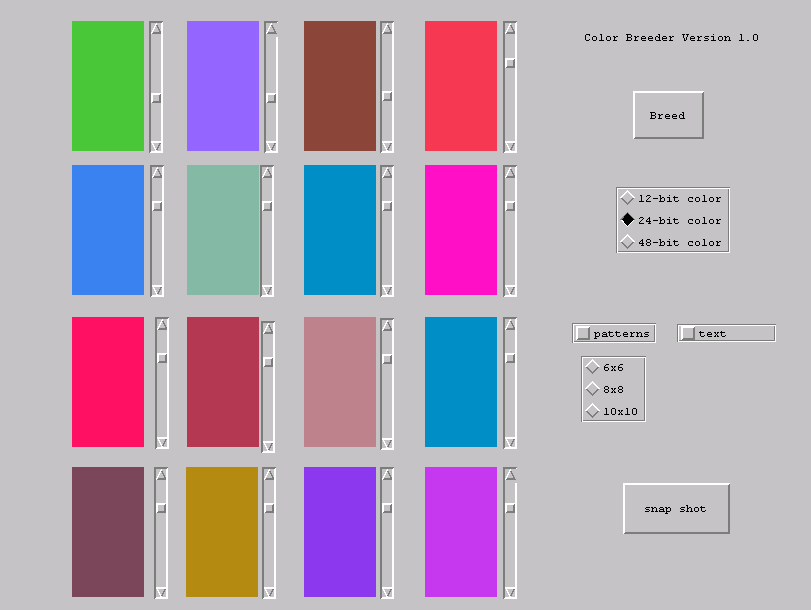
\includegraphics[width=4.0in,height=3.0in]{ub-img/ub-img46.png}
\end{center}

{\sffamily\bfseries Figure 17-2:}
{\sffamily cb - a genetic algorithm for picking colors.}



\subsection*{Breeding textures}

The user can turn on bi-level patterns of the form: \texttt{\textit{width,
\#data}} as described in Chapter 7. A bi-level pattern is tiled using
the foreground and background color to fill an area; a 1 in the
pattern denotes the foreground, and a 0 denotes the background. The
patterns come in three resolutions: 8x8, 10x10,
and 12x12. In low resolutions it is hard to find interesting patterns;
in high resolution, most patterns look like a random mixture and are
hard to evolve into something more structured. Figure 17-3 (left) shows
\texttt{cb} in pattern mode.

\bigskip

\noindent 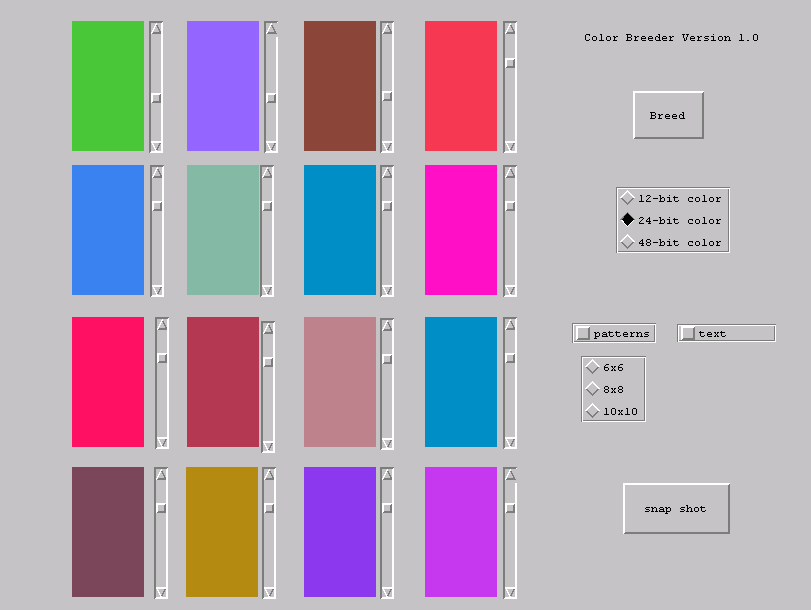
\includegraphics[width=3.125in,height=2.62in]{ub-img/ub-img47.png}
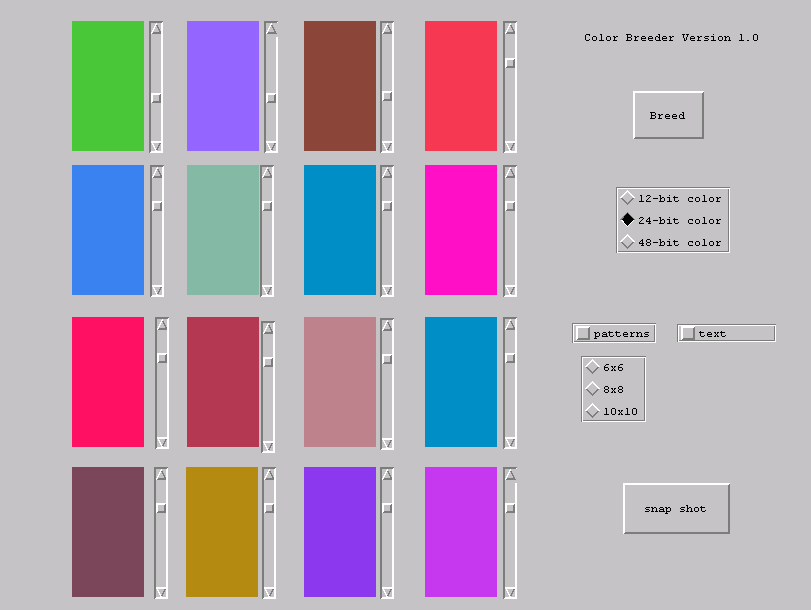
\includegraphics[width=3.125in,height=2.62in]{ub-img/ub-img48.png}

{\sffamily\bfseries Figure 17-3:}
{\sffamily \texttt{cb} in pattern mode (left) and text mode (right)}

\bigskip


The user can click on the snap shot button to create a GIF image file
that is a snapshot of the whole screen. If you left click on a color
region, the color and patterns specification will be displayed in a pop
window. For the sake of compactness, the colors and patterns are
represented with hexadecimal strings as opposed to binary strings. 

\section{Picking Colors for Text Displays}

Perhaps the most fun use of \texttt{cb} is to pick colors for your Web
pages. Figure 17-3 (right) is a snapshot of \texttt{cb} in text mode.
In text mode with 24-bit color, the user can right click on a color
region to generate a sample HTML document such as the one shown in
Figure 17-4 that demonstrates how to incorporate the selected color
combination inside of a Web page. It is also possible to get the
hexadecimal representation of a pattern or a color by right clicking on
it.

\begin{center}
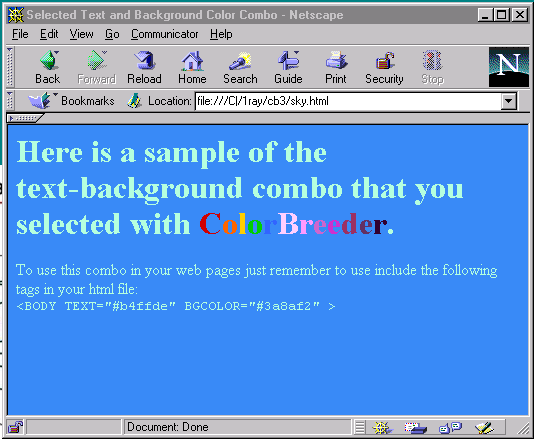
\includegraphics[width=3.7256in,height=3.0047in]{ub-img/ub-img49.png}
\end{center}

{\sffamily\bfseries Figure 17-4:}
{\sffamily A sample HTML page generated by \texttt{cb}}

\section*{Summary}

GAs are a branch of evolutionary computation that allow a
general-purpose optimization technique. The three main GA operations
are selection, mating, and mutation. Object-oriented techniques enable
a generic GA engine that can be adapted to a large variety of problems.
By making the engine very general purpose it is possible to create
applications with novel properties like using user preferences to set
the fitness of a color! 

